\begin{figure}[H]
  \centering
  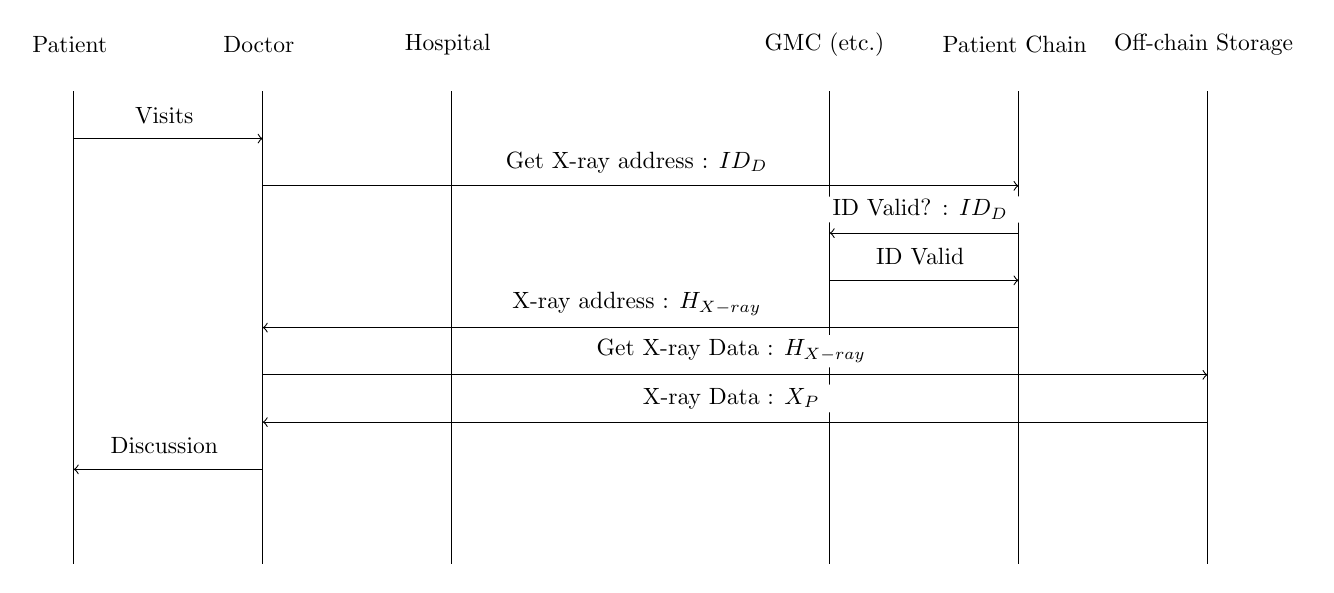
\begin{tikzpicture}[scale = 0.6, every node/.style={scale = 0.85}, every node/.append style={fill = white, rounded corners = 2pt, inner sep = 2pt, align = center}]

  % Lines
  \draw (4, 10) -- (4, 20);
  \draw (8, 10) -- (8, 20);
  \draw (12, 10) -- (12, 20);
  \draw (20, 10) -- (20, 20);
  \draw (24, 10) -- (24, 20);
  \draw (28, 10) -- (28, 20);

  % Headings
  \node at (4, 21) { Patient };
  \node at (8, 21) { Doctor };
  \node at (12, 21) { Hospital };
  \node at (20, 21) { GMC (etc.) };
  \node at (24, 21) { Patient Chain };
  \node at (28, 21) { Off-chain Storage };

  % Arrows
  \node at (6, 19.5) { Visits };
  \draw [ -> ] (4, 19) -- (8, 19);

  \node at (16, 18.5) { Get X-ray address : $ID_{D}$ };
  \draw [ -> ] (8, 18) -- (24, 18);

  \node at (22, 17.5) { ID Valid? : $ID_{D}$ };
  \draw [ -> ] (24, 17) -- (20, 17);

  \node at (22, 16.5) { ID Valid \checkmark };
  \draw [ -> ] (20, 16) -- (24, 16);

  \node at (16, 15.5) { X-ray address : $H_{\text{X-ray}}$ };
  \draw [ -> ] (24, 15) -- (8, 15);

  \node at (18, 14.5) { Get X-ray Data : $H_{\text{X-ray}}$ };
  \draw [ -> ] (8, 14) -- (28, 14);

  \node at (18, 13.5) { X-ray Data : $X_{P}$ };
  \draw [ -> ] (28, 13) -- (8, 13);
  
  \node at (6, 12.5) { Discussion };
  \draw [ -> ] (8, 12) -- (4, 12);

  \end{tikzpicture}
  \caption{Doctor views X-ray with patient}{
  	The patient visits the doctor to discuss their X-ray results. The doctor gets the latest version (address / hash) of their X-ray data from their record and using this gets the X-ray data itself from off-chain storage. The doctor is then able to discuss the results with the patient (and make further edits - \textit{not shown}.
  }
  \label{fig:user_story_03}
\end{figure}
